\documentclass{article}
\usepackage[utf8]{inputenc}
\usepackage{graphicx}
\usepackage[titletoc]{appendix}
\begin{document}
\begin{titlepage}
	\author{Lars Gaidzik und Lukas Mahr} 
	\title{Stundenplanapp der Hochschule Hof}
	\date{} 
	\maketitle
\end{titlepage}
\tableofcontents
\newpage
\section{Vorwort}
Im Folgenden werden alle bereits verfügbaren Funktionen der App vorgestellt, die im Wintersemester 2015/16 im Fach Aspekte der Android-Programmierung erstellt wurden. 
Des Weiteren wird auf Änderungen eingegangen, die noch vorgenommen werden können. Im Anhang sind Screenshots der aktuellen App enthalten.
\section{Aktueller Funktionsumfang}
\begin{itemize}
\item Stundenplan

\item Stundenplanänderungen

\item Speiseplan

\item Raumsuche

\item Notenbekanntgabe

\item Notenblatt
\end{itemize}
Für die Raumsuche, Notenbekanntgabe und das Notenblatt wird der Hochschul-Benutzername und das dazugehörige Passwort benötigt. 
Dieses wird in den Einstellungen der App hinterlegt. Hier wird auch der Studiengang für den Stundenplan gewählt. 
Für den Speiseplan kann der Tarif (Mitarbeiter, Student, ...) angegeben werden.

\section{Neue Anforderungen}
\subsection{Programmier-Schnittstelle}
\label{schnittstelle}

Aktuell müssen alle Informationen zum Studium, Stundenplan, Stundenplanänderungen, Noten, u.v.a.m, aus dem Quellcode der Hochschulwebsite geladen werden.
Diese Daten sollen in der App angezeigt werden, dazu müssen mühsam die Portale der Hochschule, des Studentenwerks und des Primuss-Portals eingelesen werden. 
Dieses Verfahren ist jedoch aus unserer Erfahrung heraus sehr fehleranfällig und ineffizient. 

Des Weiteren kann es dadurch sehr leicht passieren, dass durch eine Anpassung an den Websites die Funktion innerhalb der App nicht mehr funktioniert und auch angepasst werden muss. 
\\
Einfacher, auch für zukünftige Anwendungen, ist eine wohldefinierte Schnittstelle unabhängig vom Aussehen der Weboberfläche. Hier sollten auch Verwaltungs-IDs mitgeführt werden, 
damit aus Programmierersicht ein-eindeutige Beziehungen zwischen den Einträgen (Objekte) herstellbar sind.

Somit könnten dann die Stundenpläne und deren Änderungen ineinander gepflegt werden und müssten nicht mehr nebeneinander dem Studenten angezeigt werden.

Diese Schnittstelle könnte auch von anderen Entwicklern genutzt werden, um beispielsweise ein App für iOS und WindowsPhone zu erstellen. 


\subsection{Stundenplanänderungen in den Stundenplan integrieren}
\label{integrieren}
Aktuell reicht es nicht, in den Stundenplan zu blicken, um sicher zu wissen, wo und wann eine Vorlesung stattfindet. 
Es müssen zusätzlich die separat dargestellten Stundenplanänderungen täglich (oder sogar vor jeder Vorlesung) geprüft werden. 
Deutlich effizienter wäre es, diese Änderungen direkt in dem Stundenplan für die aktuelle Woche zu integrieren. \\

Dafür ist es aus technischer Sicht notwendig, die verschiedenen Vorlesungen und dazugehörige Änderungen mit eindeutigen IDs zu versehen,
 um einen Zusammenhang zwischen den Änderungen und der jeweiligen Vorlesung herstellen zu können.

\subsection{Stundenplan filtern}

Besonders in den höheren Semestern, in denen aus einem großen Angebot von Modulen nur noch wenige Fächer belegt werden müssen, 
ist der Stundenplan momentan sehr unübersichtlich. Auch das Feedback einiger Kommilitonen, die die App bereits testen durften, hat gezeigt, 
dass eine Filterfunktion nicht nur auf den gesamten Studiengang sondern im Speziellen auf einige ausgwählte Fächer (FWM, AWM) sehr nützlich wäre. 
Dann könnte der Anwender elegant seine persönliche Ansicht auf die für ihn relevanten Vorlesungen einschränken. \\

Technisch wäre hier auch sehr hilfreich, das Vorgehen mit Hilfe der eineindeutigen IDs, wie im Punkt \ref{integrieren} vorgestellten Änderung, umzusetzen.

\subsection{Benachrichtigung bei neuen Noten}
Auf Wunsch wäre es möglich, die Notenbekanntgabe regelmäßig auf Änderungen zu prüfen und damit informiert zu werden, wenn eine neue Note zur Verfügung steht. 
Das würde vielen Studenten das manuelle Prüfen der Notenbekanntgabe (was erfahrungsgemäß sehr häufig durchgeführt wird) ersparen.\\
Technisch wäre dies ohne weitere Anpassungen umsetzbar.

\subsection{Raumbezogenen Stundenplan anzeigen}
Denkbar wäre das Anbringen von QR-Codes, NFC-Tags oder Beacons an jedem Vorlesungsraum der Hochschule. 
Damit könnte man einen Raum identifizieren, wenn man beispielsweise davor steht und einen Belegplan des Raums anzeigen.\\

Technisch wären hierfür die bereits erwähnten QR-Codes, etc. nötig. Außerdem bräuchte man erweiterten Zugriff auf die 
Stundenplan-Informationen. Daher wäre hierfür die bereits im Punkt \ref{schnittstelle} vorgestellte Programmier-Schnittstelle nötig.

\newpage
\section{Screenshots}
\begin{appendices}
	\begin{figure}
		\centering
		
\includegraphics[width=0.7\linewidth]{appendix/stundenplan}
		\caption{Stundenplan}
	\end{figure}
	\begin{figure}
		\centering
		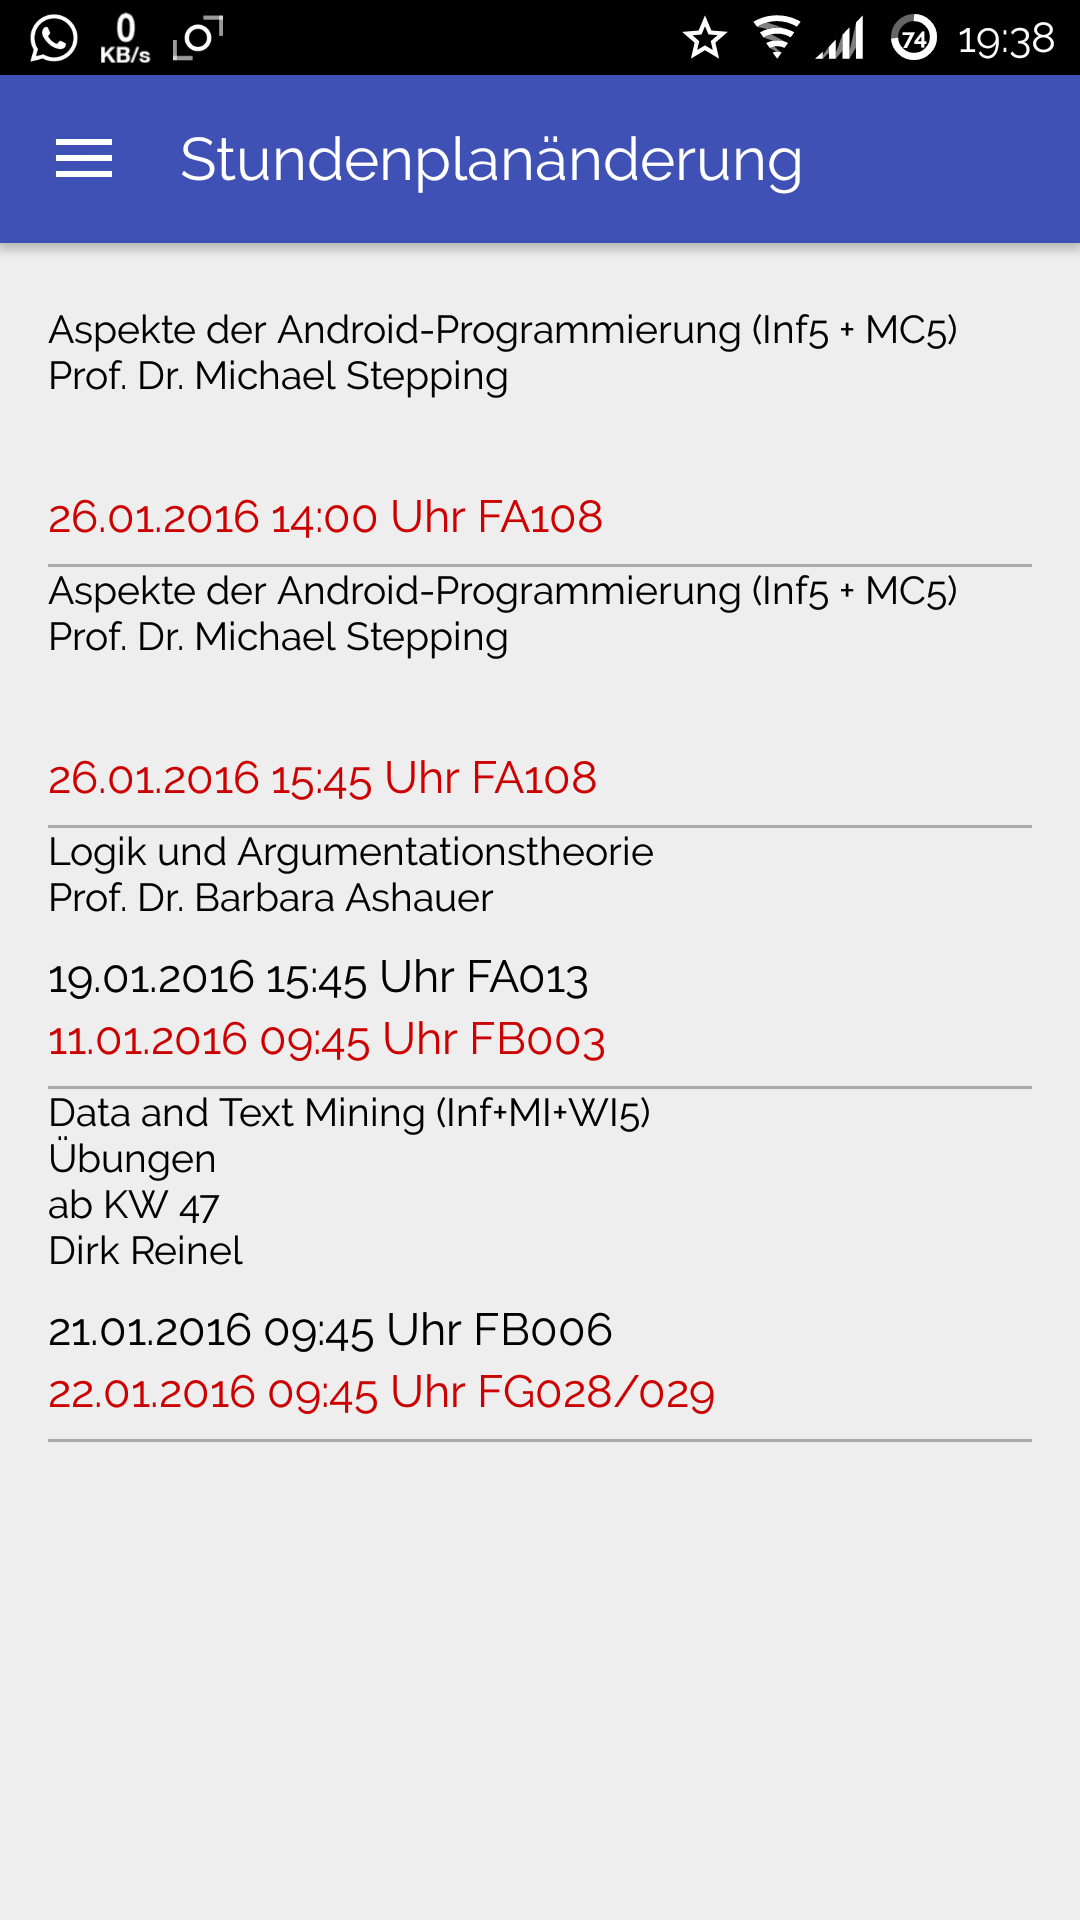
\includegraphics[width=0.7\linewidth]{appendix/aenderung}
		\caption{Stundenplanänderungen}
	\end{figure}
	\begin{figure}
		\centering
		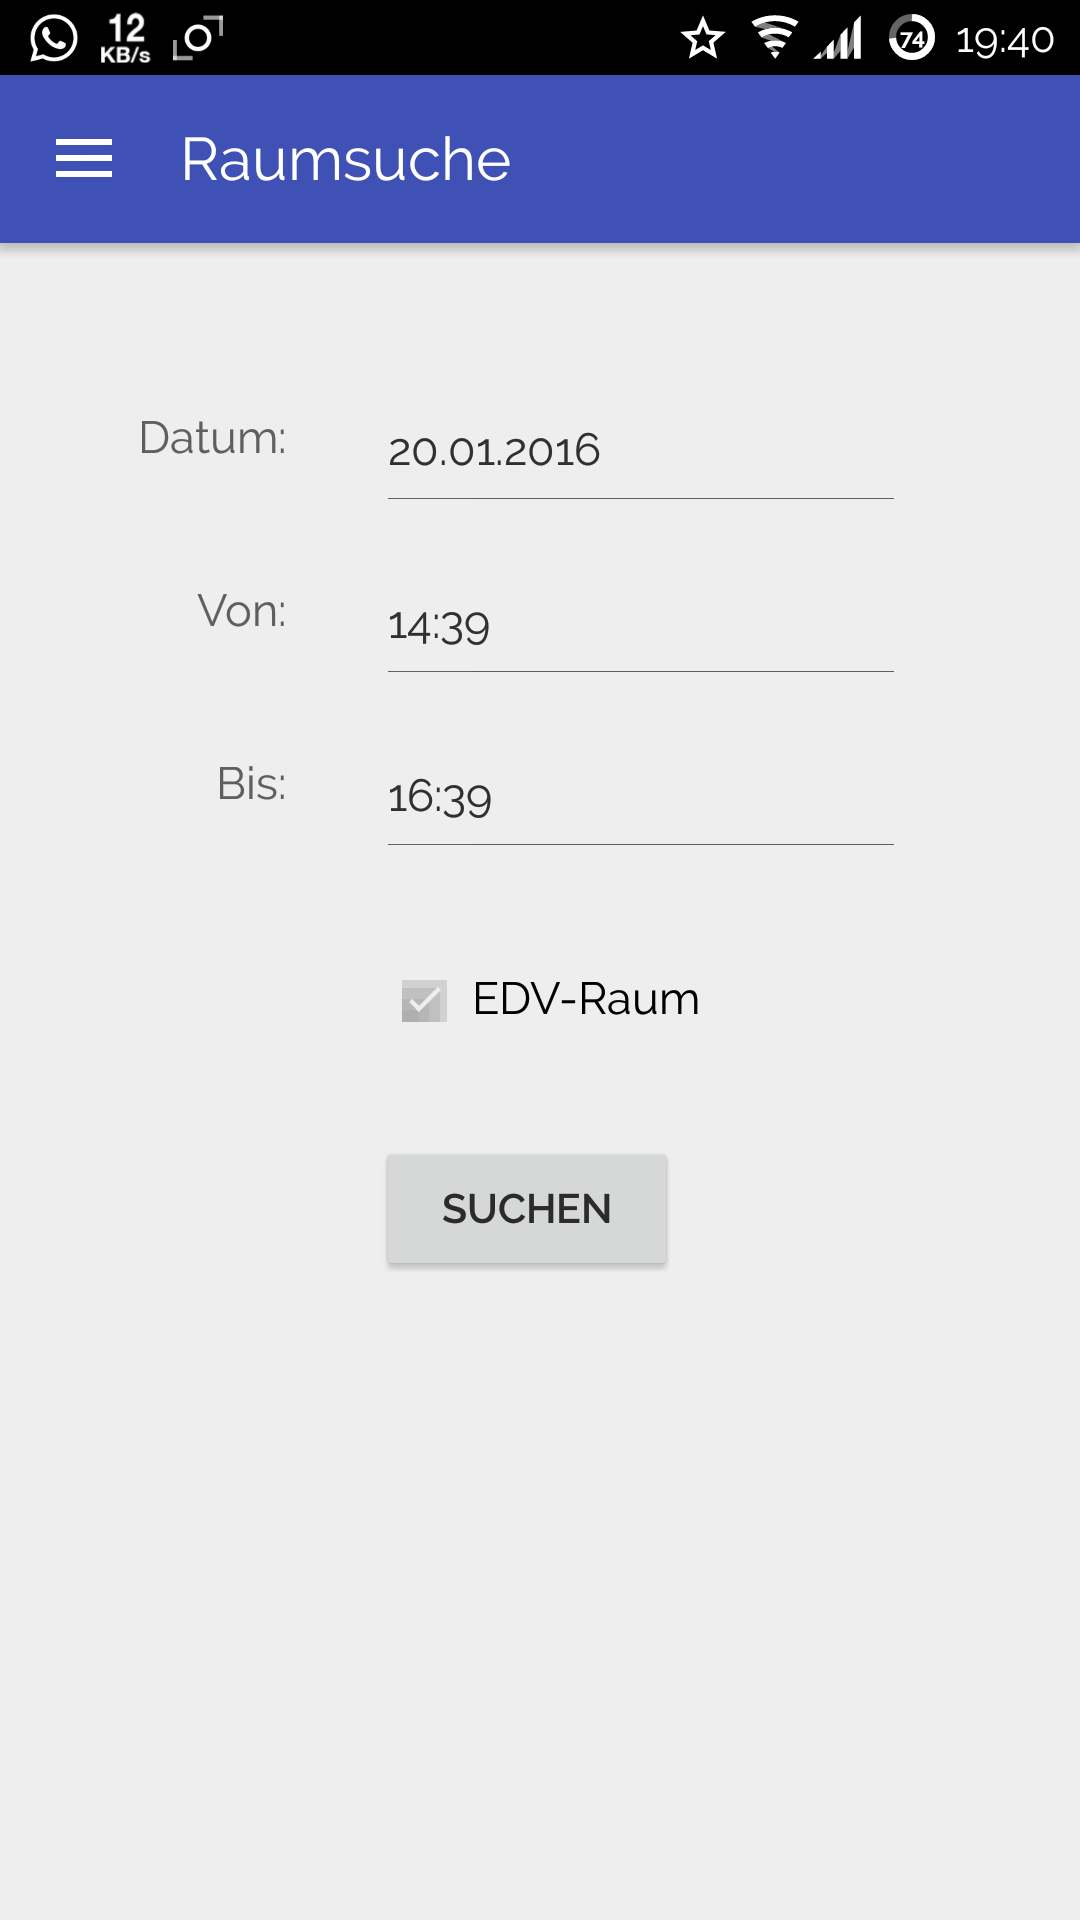
\includegraphics[width=0.7\linewidth]{appendix/raumsuche}
		\caption{Suchdialog der Raumsuche}
	\end{figure}
	\begin{figure}
		\centering
		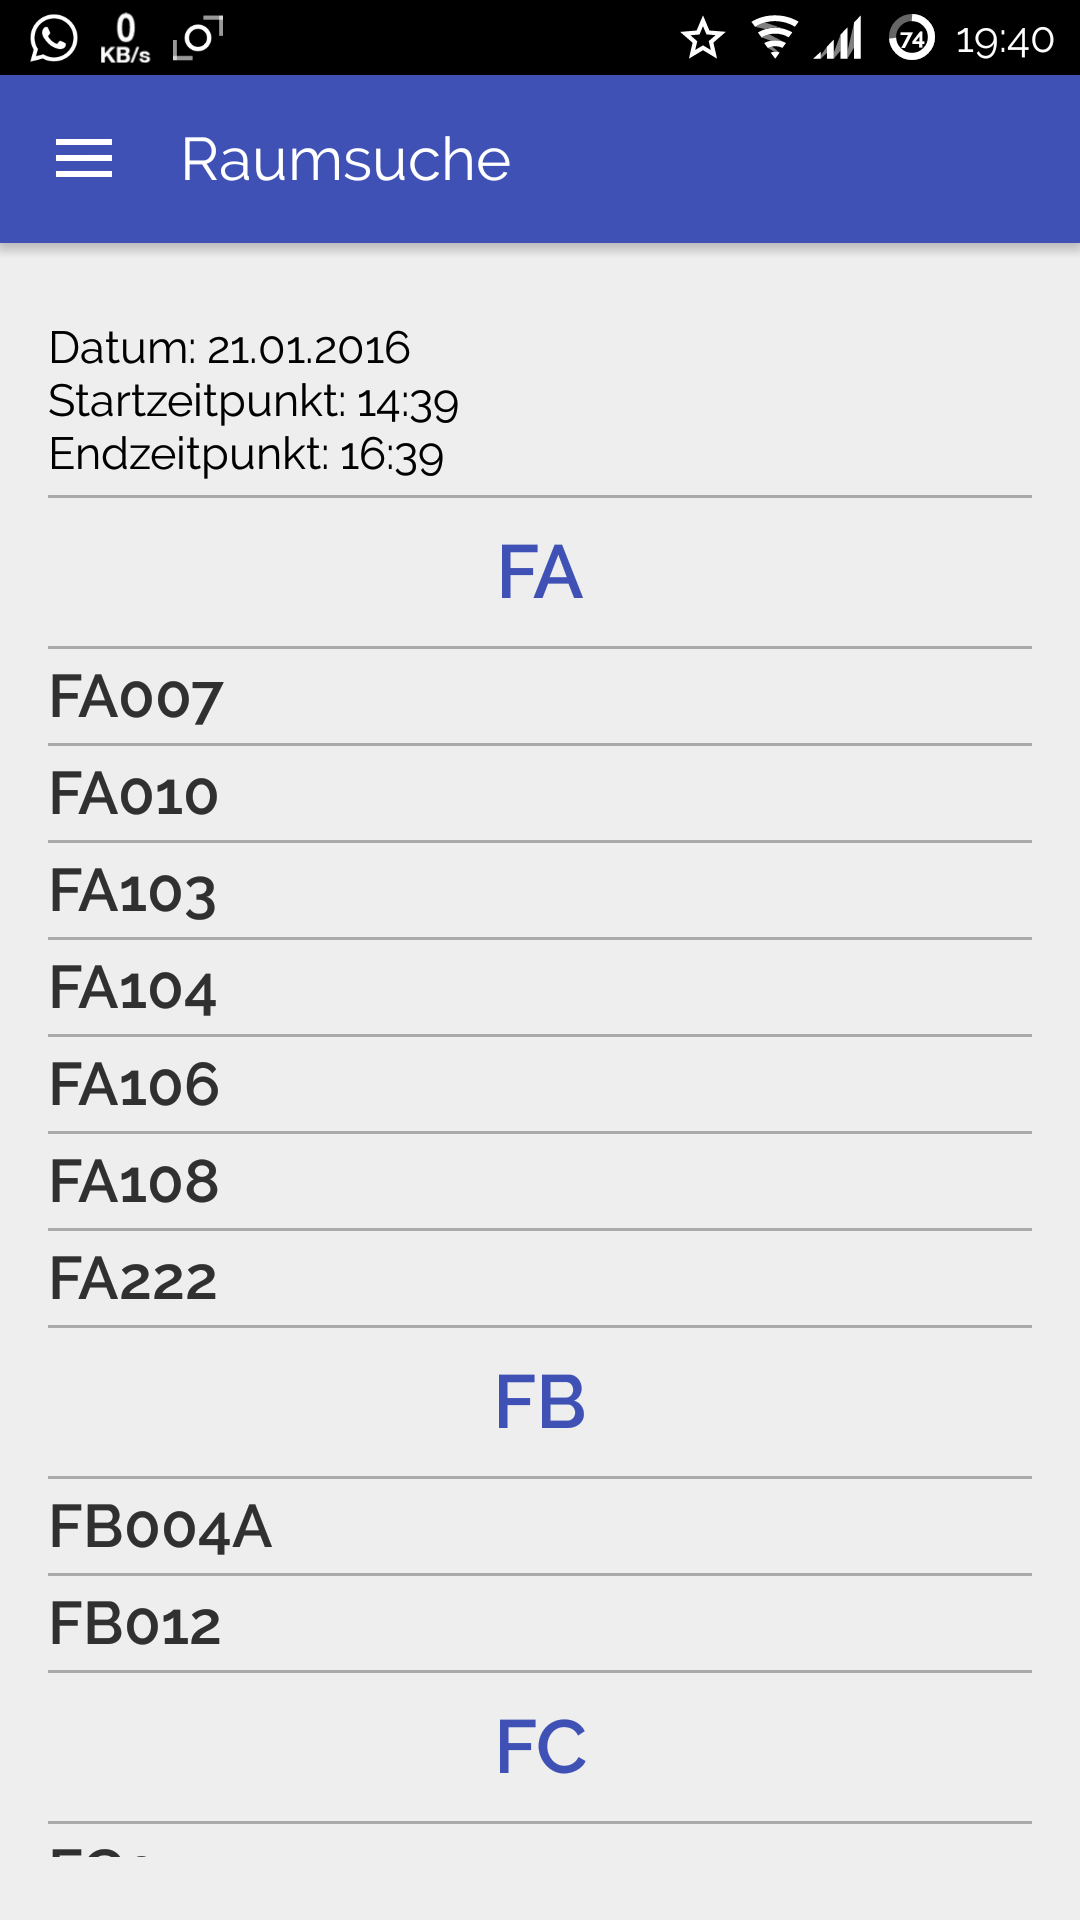
\includegraphics[width=0.7\linewidth]{appendix/raumliste}
		\caption{Raumliste mit den freien Räumen}
	\end{figure}
	\begin{figure}
		\centering
		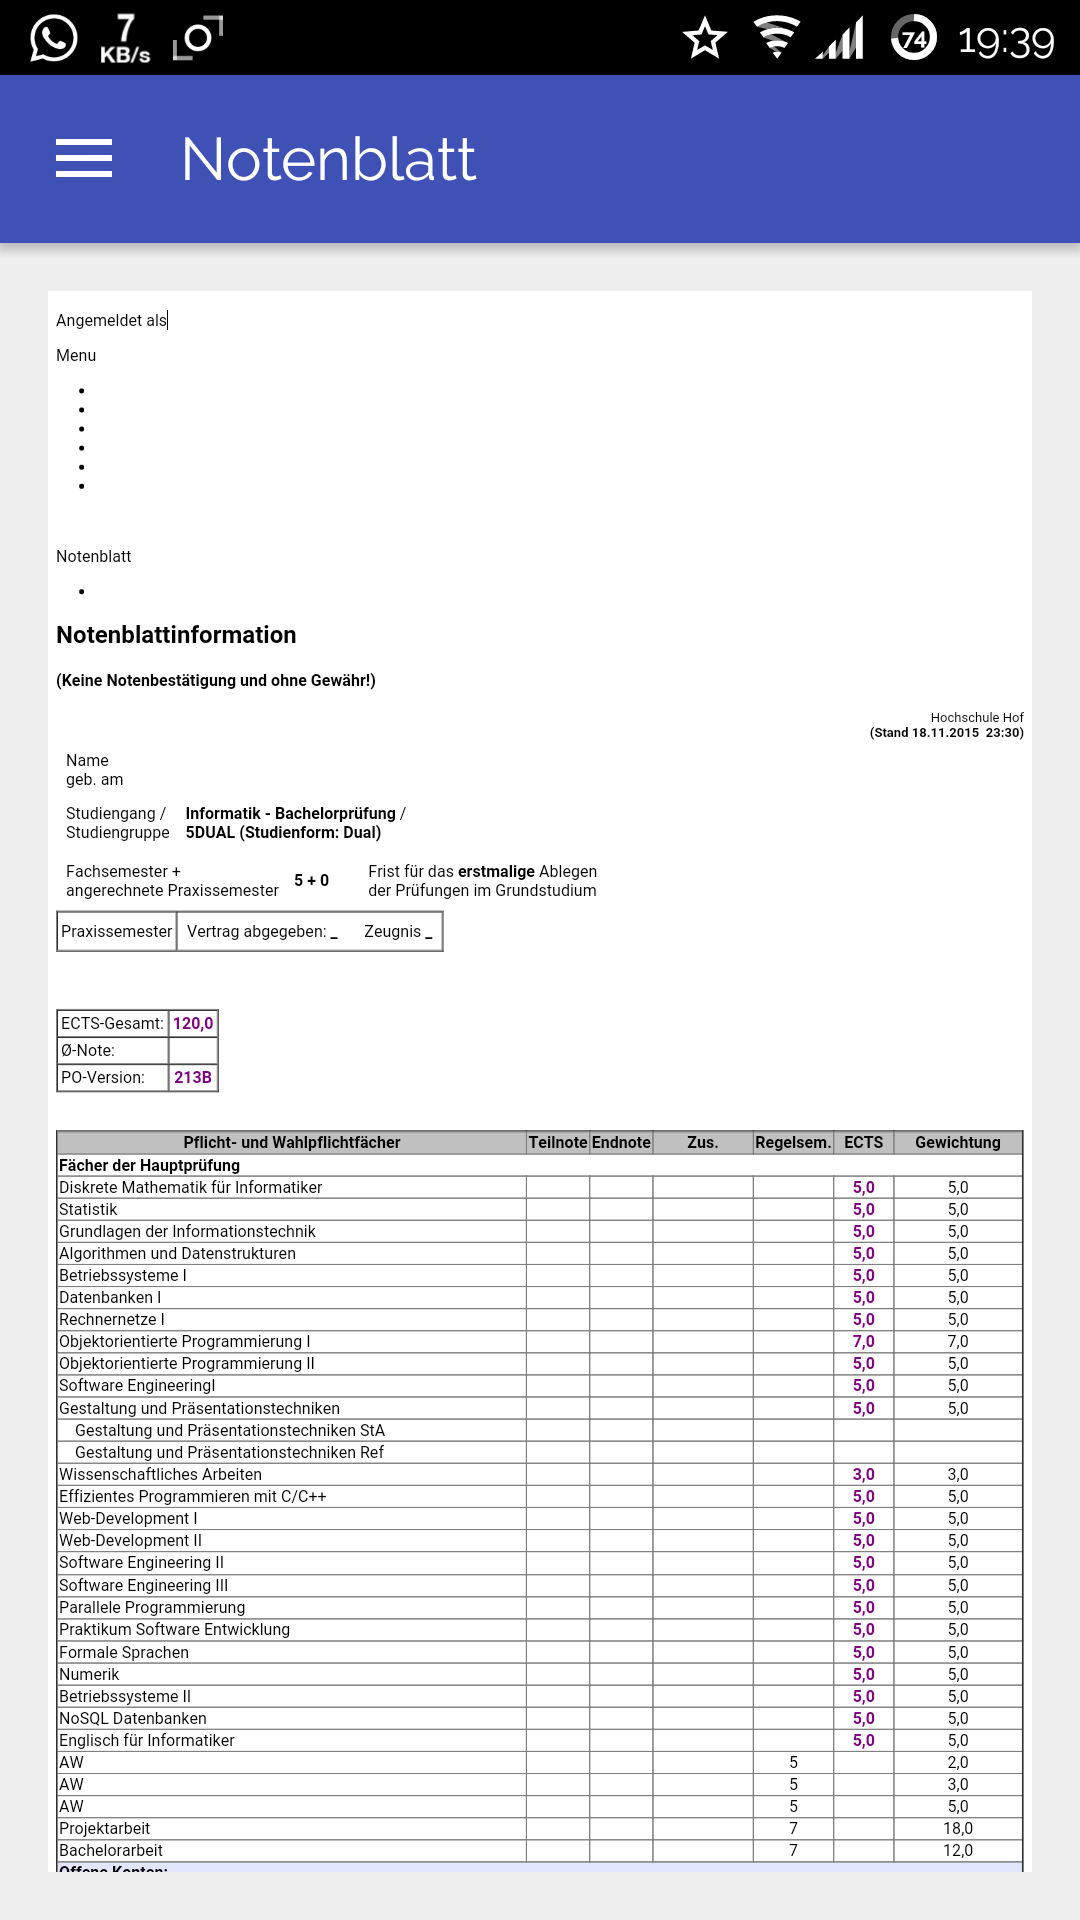
\includegraphics[width=0.7\linewidth]{appendix/notenblatt}
		\caption{Übersicht über alle Noten im Studium}
	\end{figure}
	\begin{figure}
		\centering
		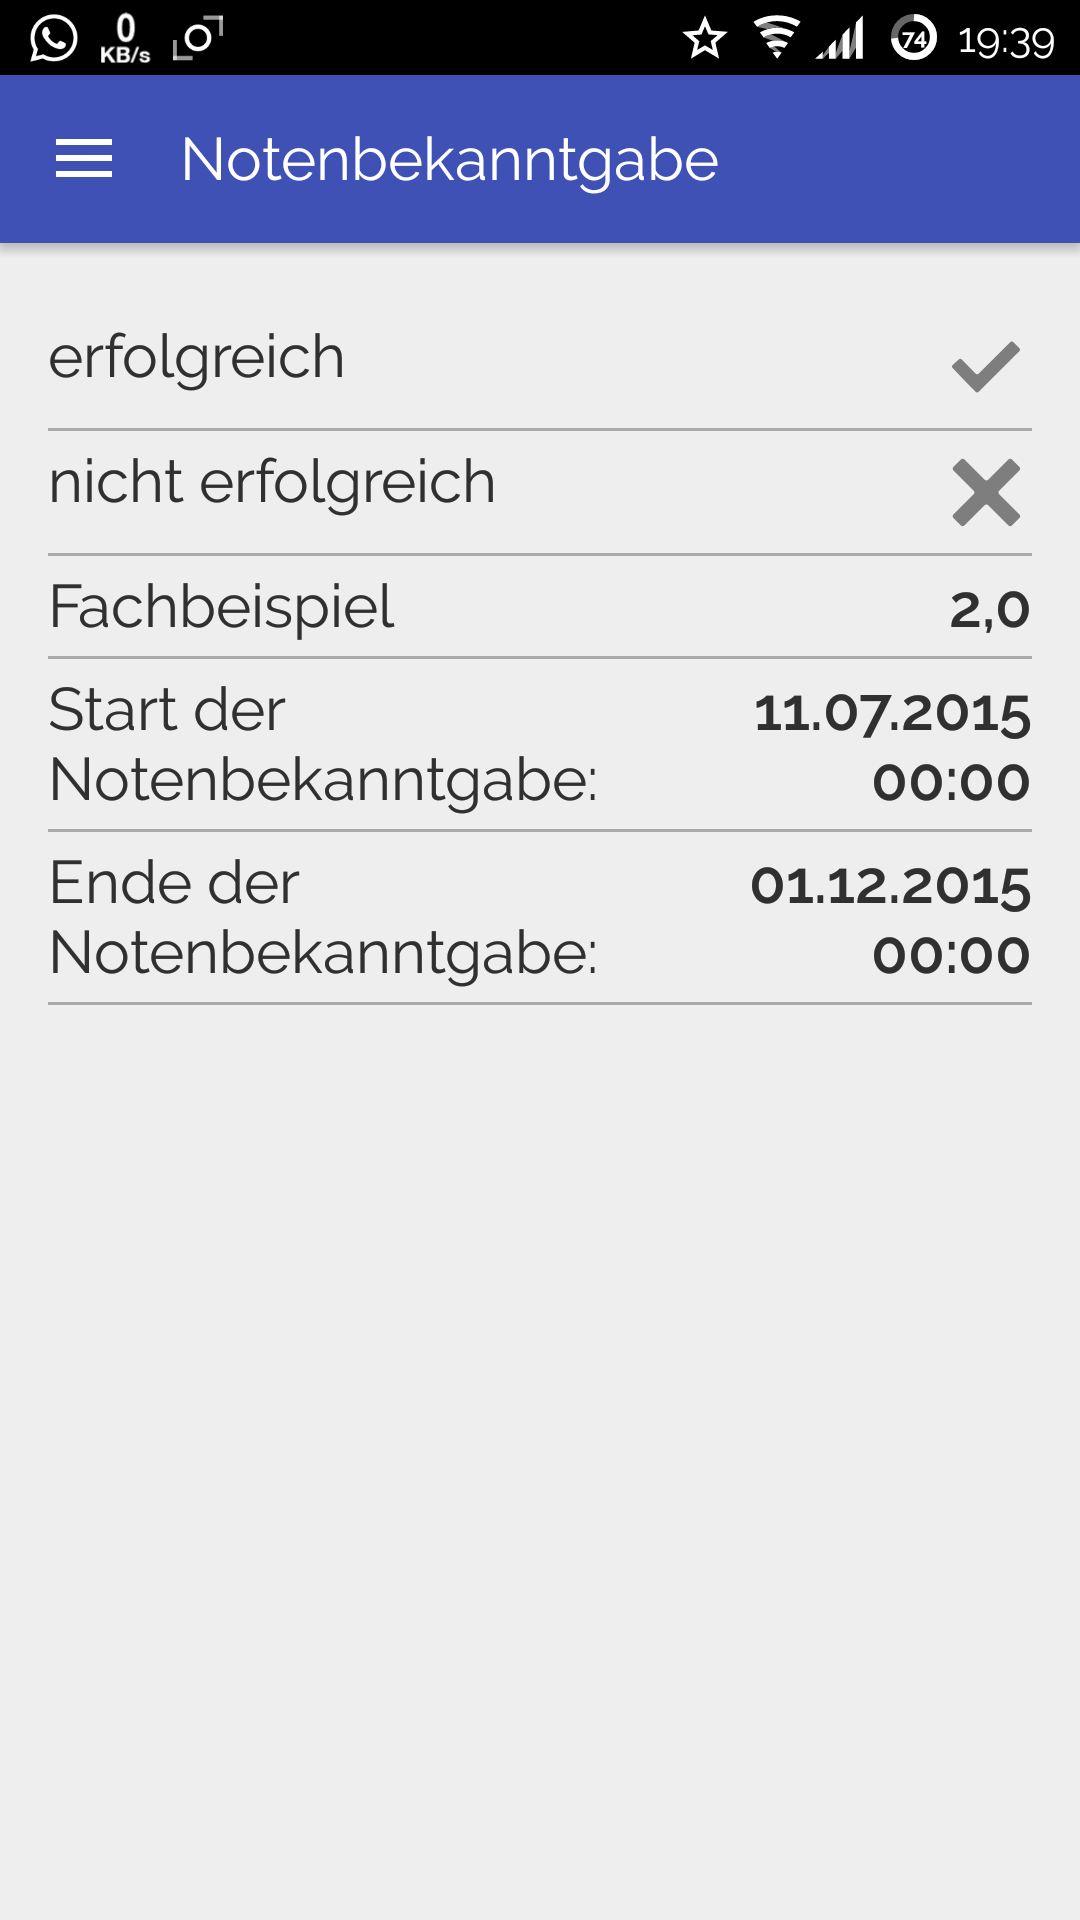
\includegraphics[width=0.7\linewidth]{appendix/notenbekanntgabe}
		\caption{Notenbekanntgabe des aktuellen Semesters}
	\end{figure}
	\begin{figure}
		\centering
		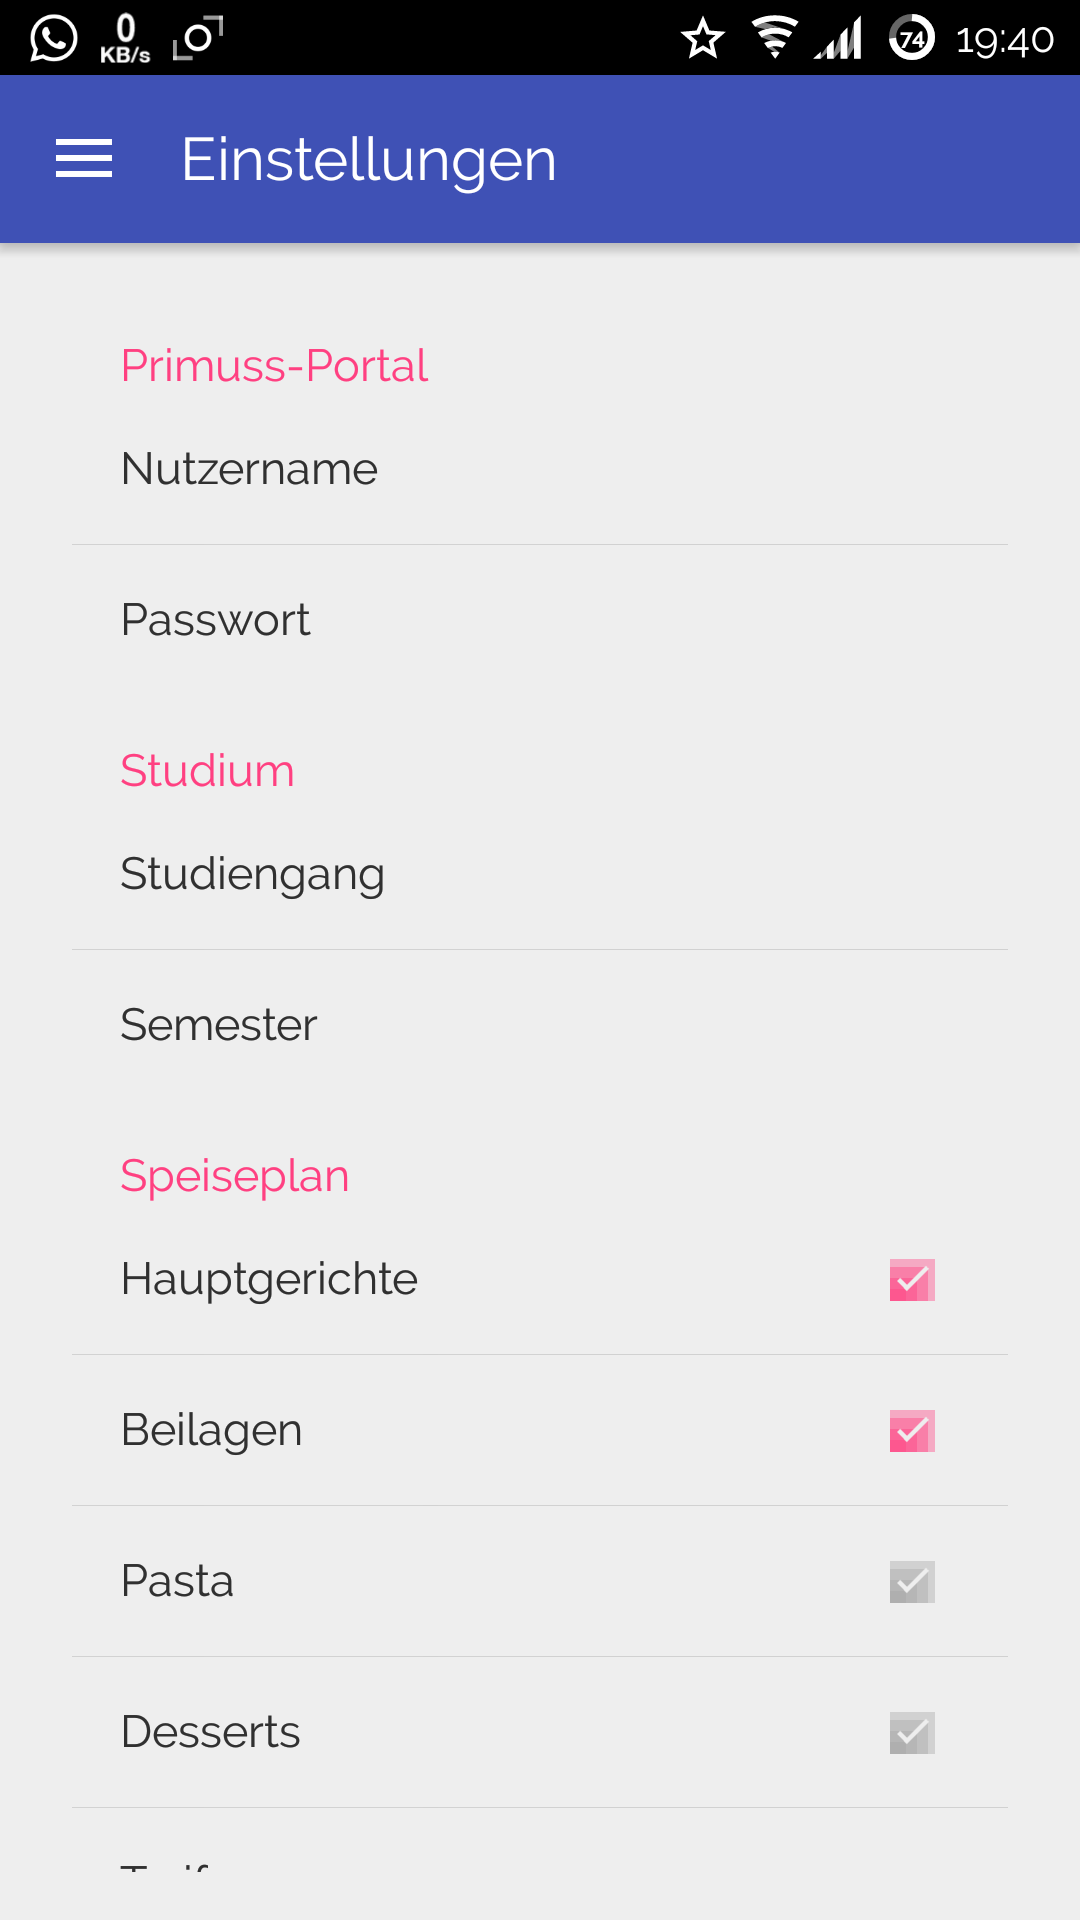
\includegraphics[width=0.7\linewidth]{appendix/einstellungen}
		\caption{Einstellungen}
	\end{figure}
	\begin{figure}
		\centering
		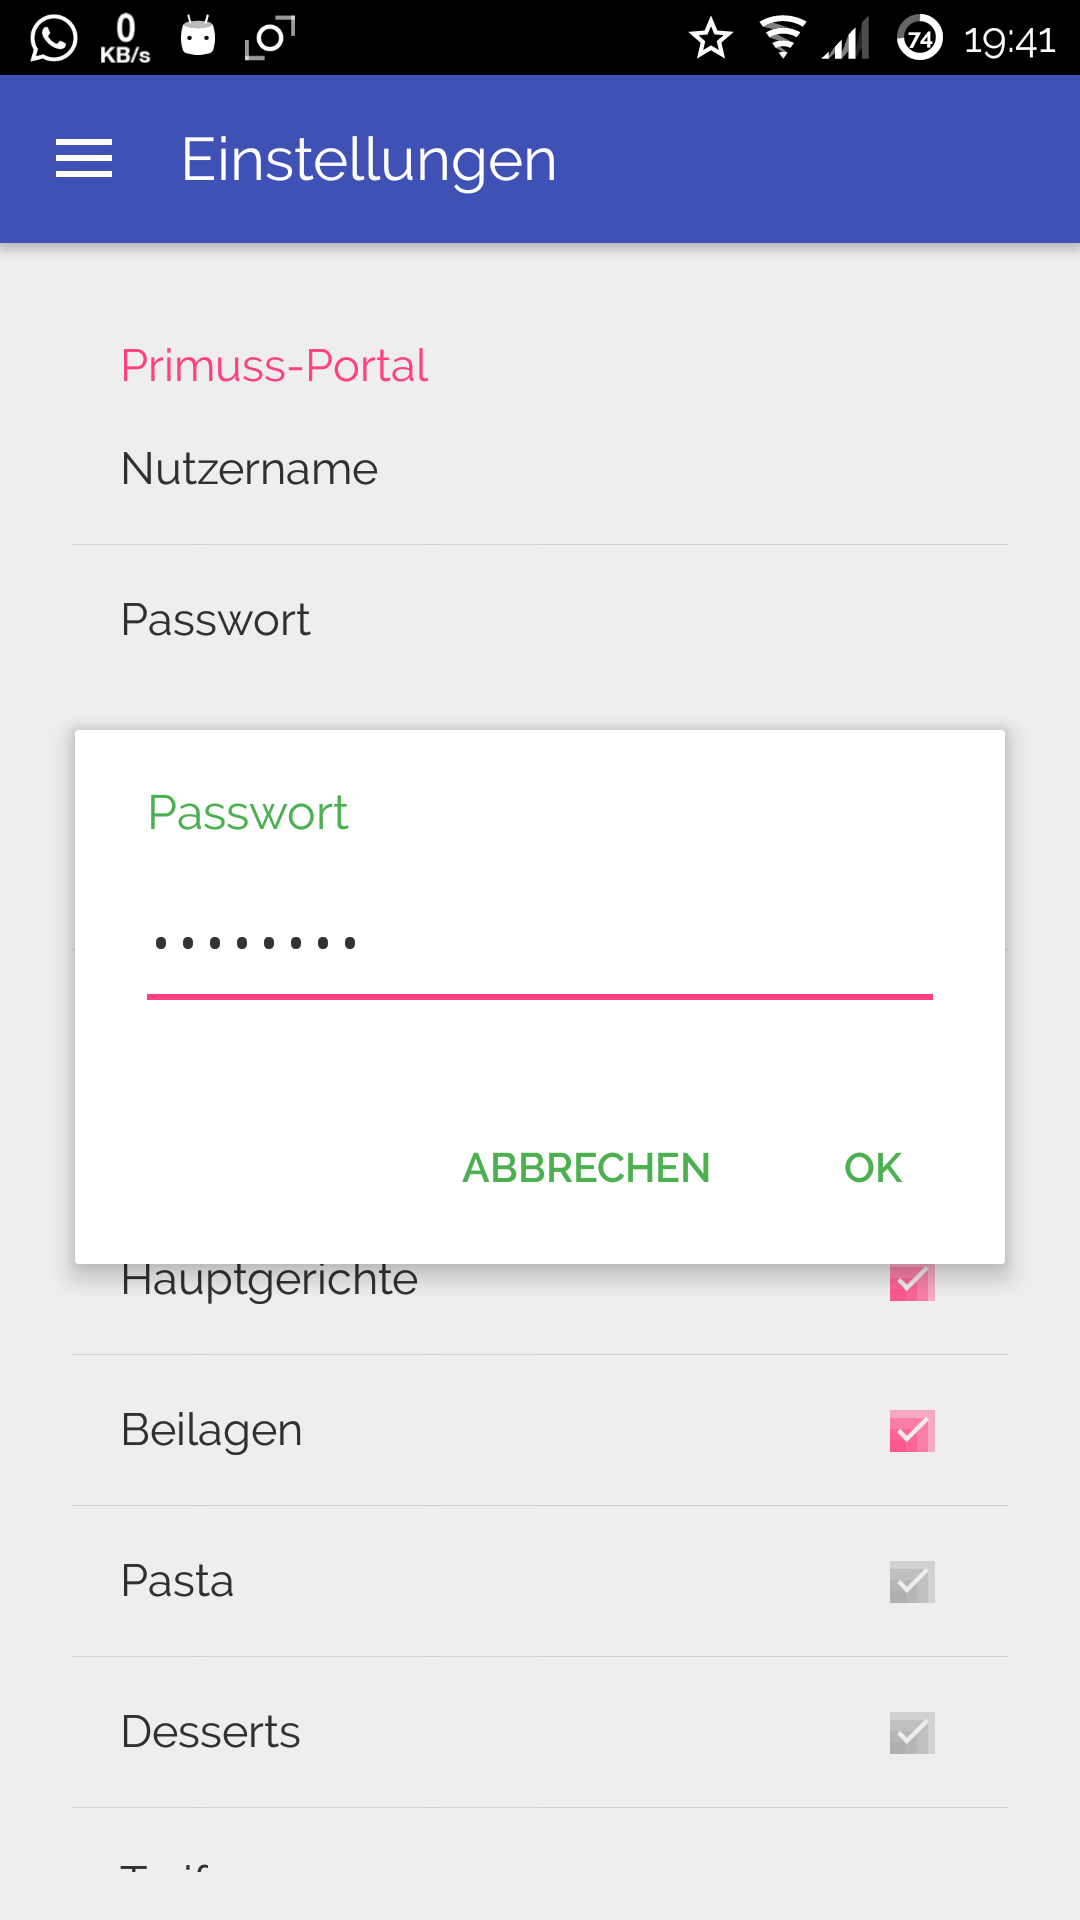
\includegraphics[width=0.7\linewidth]{appendix/einstellungen_pw}
		\caption{Einstellungen - Passwort eingeben}
	\end{figure}
	\begin{figure}
		\centering
		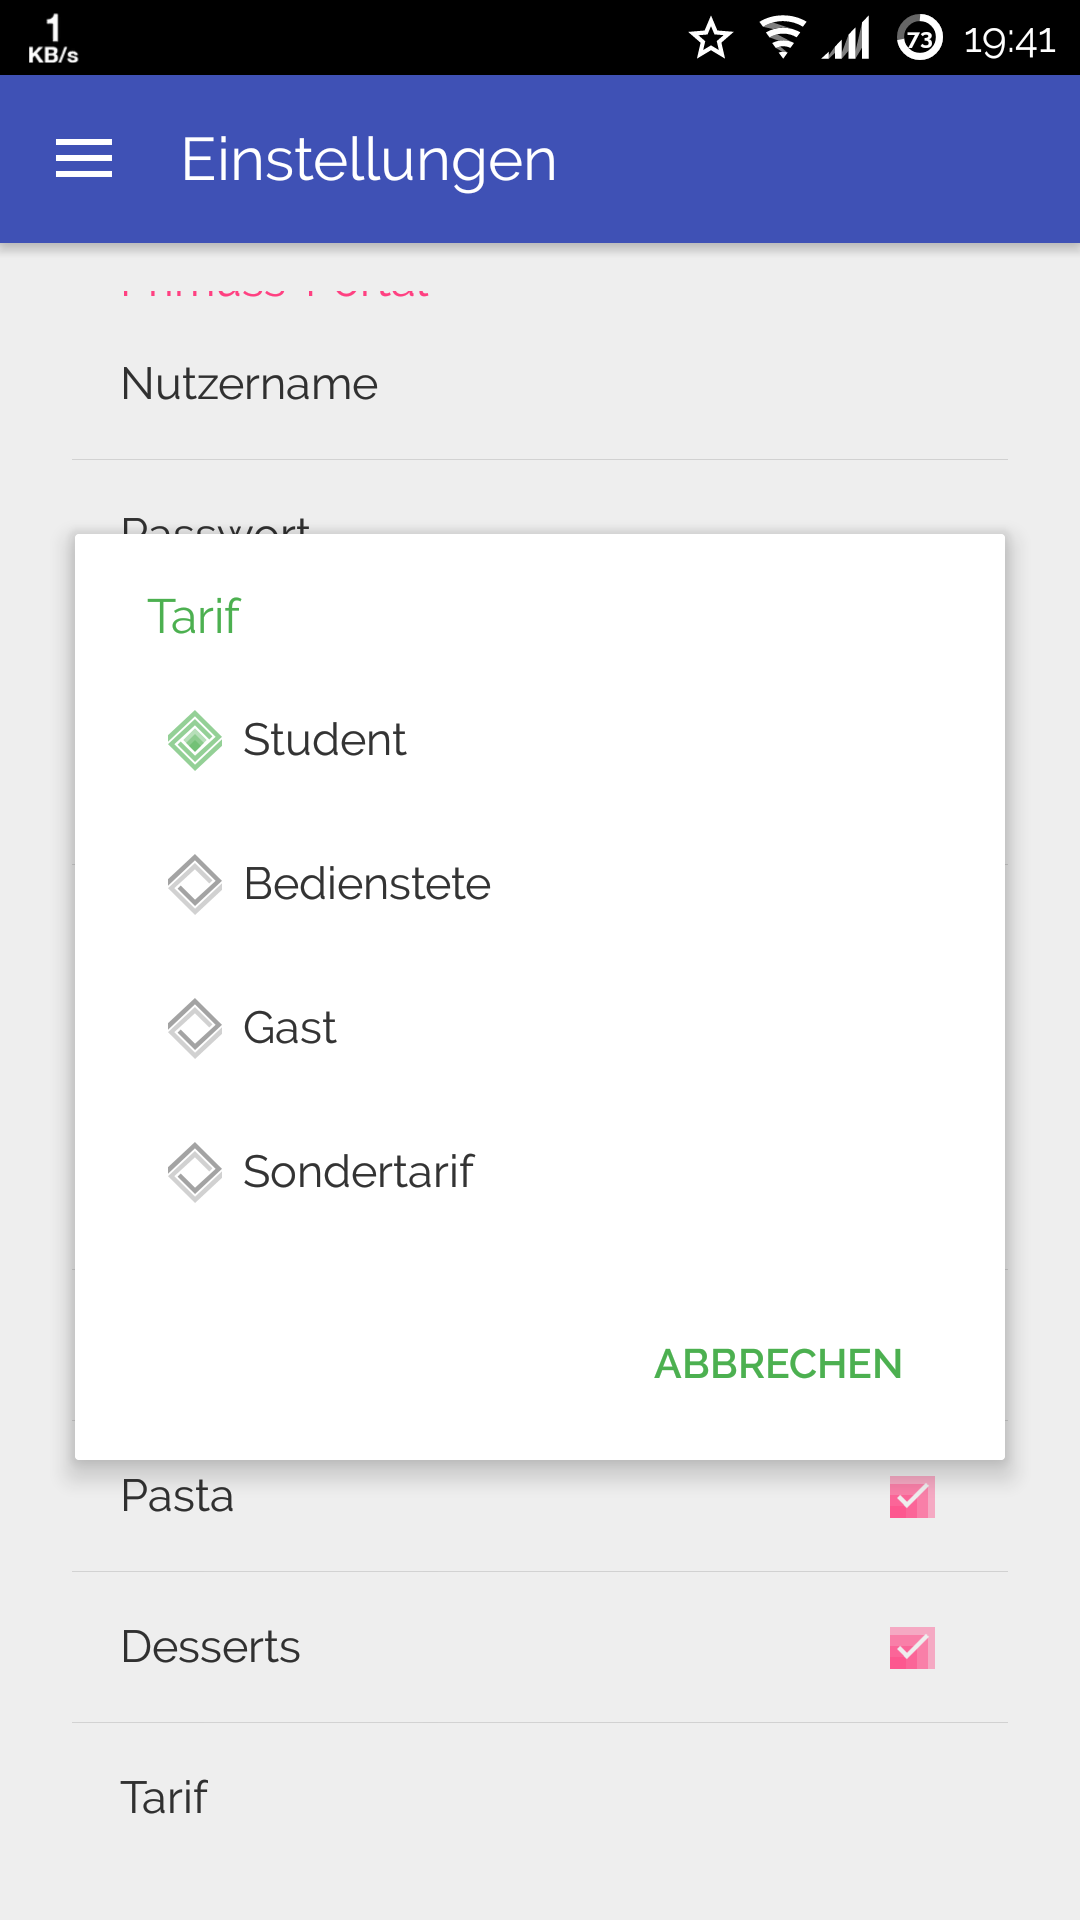
\includegraphics[width=0.7\linewidth]{appendix/einstellungen_tarif}
		\caption{Einstellungen - Tarif wählen}
	\end{figure}
	
\end{appendices}


\end{document}
